\documentclass[11pt,
  letterpaper,
  openany,
  toc=bibliography,
  idxtotoc,
  bookmarks]{labbook}

\usepackage[utf8]{inputenc}
\usepackage[T1]{fontenc}
\usepackage[spanish]{babel}

\usepackage[margin=2.5cm]{geometry}
\usepackage{microtype}
\usepackage{graphicx}
\usepackage{amsmath,amssymb}
\usepackage{csquotes}
\usepackage{booktabs}
\usepackage{enumitem}
\usepackage{authblk}
\usepackage[spanish]{cleveref}
\usepackage[dvipsnames]{xcolor}
\usepackage{pgfplotstable}
\usepackage{siunitx}

\pgfplotsset{compat=1.18}
\pgfkeys{/pgf/number format/1000 sep={\,}}

\AtBeginDocument{\decimalpoint}
\renewcommand{\arraystretch}{1.2}
\sisetup{group-digits=true,
  group-separator={\,},
  separate-uncertainty}

\usepackage[backend=biber,style=numeric]{biblatex}
\addbibresource{./references-pre-project.bib}

\usepackage{pdfbase}
\pdfinfo{
  /Title (Osciladores Acoplados - Bitácora de Laboratorio)
  /Author (Sebastián Rodríguez, Laura Torres, Julián Ávila)
  /Creator (LaTeX with labbook class)
}

\title{\textbf{Osciladores Acoplados} \\
Bitácora de Laboratorio}
\author{Sebastian Rodríguez \and Laura Torres \and Julian Avila}
\affil{Universidad Distrital Francisco José de Caldas}
\date{}

\begin{document}

\maketitle

\tableofcontents

\labday{Miércoles 23, Abril 2025}




\labday{Jueves 24, Abril 2025}

\experiment{Planteamiento Teórico}
Se desarrolla el fundamento teórico del problema de los tres péndulos
físicos acoplados por resortes. A partir del desplazamiento angular
de cada péndulo, \(\theta_i\), se establece el sistema planteado con
sus relaciones importantes, presentado en la \cref{fig:sistema-pendulos}.

\begin{figure}[htbp!]
  \centering
  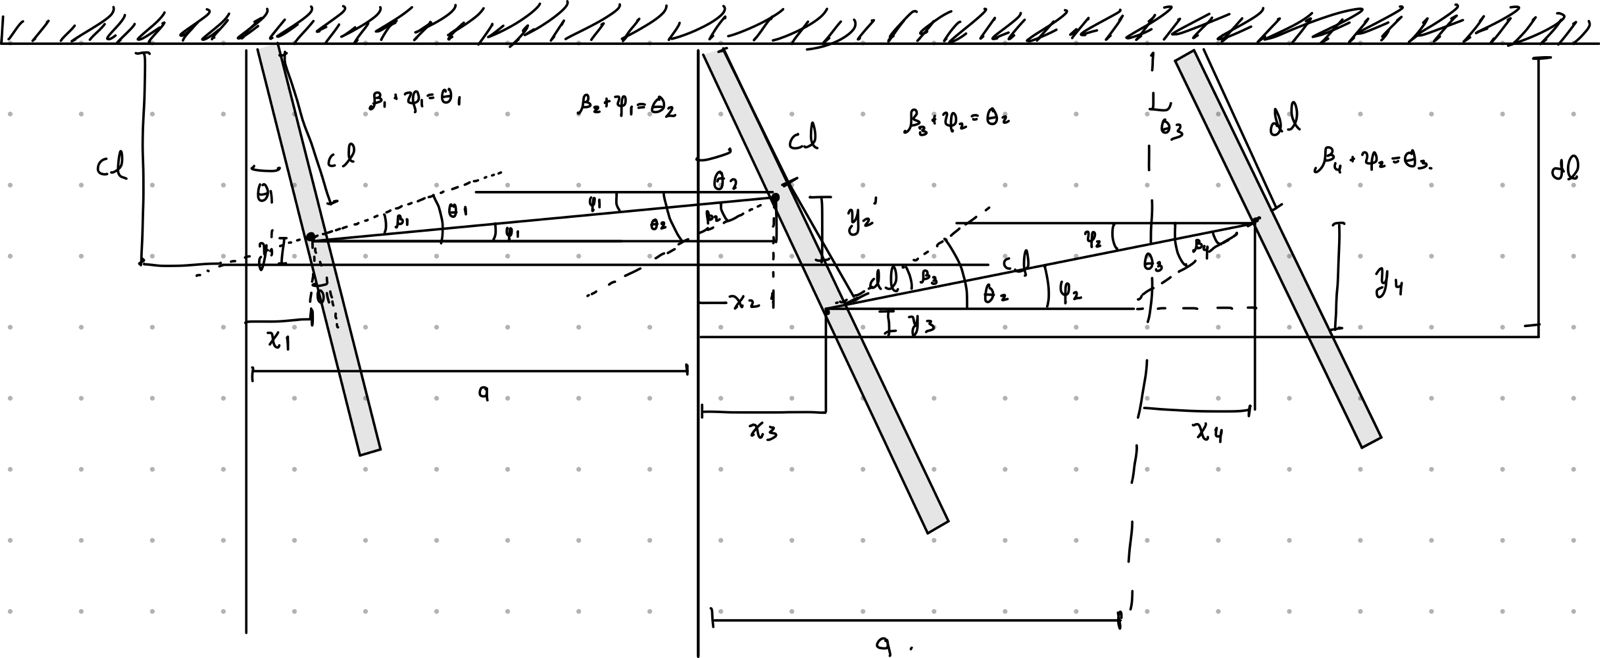
\includegraphics[width=0.8\linewidth]{Figures/IM1.jpeg}
  \caption{Sistema de tres péndulos físicos acoplados por resortes.}
  \label{fig:sistema-pendulos}
\end{figure}

Considerando el desplazamiento angular de cada péndulo, se determina
la suma de los torques que actúan sobre cada uno para derivar el
sistema de ecuaciones del movimiento.

La distancia \( a \) es la separación entre cada péndulo. \( cl \) es
la distancia a la cual se acoplan los péndulos 1 y 2 por medio del
resorte con constante \( k_1 \), mientras que \( dl \) es la distancia
de acople entre 2 y 3 por medio del resorte con constante \( k_2 \).
Los \(y_{\text{cm}_i}\) corresponden a la distancia desde el punto de
giro al centro de masa. De esta forma, el torque restaurador
gravitacional está relacionado con \(m_i g y_{\text{cm}_i} \sin{\theta_i}\).

Para las interacciones generadas por los resortes, se asume que
obedecen a la ley de Hooke lineal y que actúan a lo largo de una
línea de acción horizontal. De esta forma, se aplicará una
aproximación lineal a todos los términos angulares no lineales.

La sumatoria de torques para cada péndulo genera el siguiente
sistema de ecuaciones diferenciales:

\begin{equation}
  \begin{aligned}
    \ddot{\theta}_1 =\; &
    -\theta_1 \left[ \frac{k_1 (cl)^2 + y_{\text{cm}_1} m_1 g}{I_1} \right]
    + \theta_2 \left( \frac{k_1 (cl)^2}{I_1} \right) \\[0.5em]
    \ddot{\theta}_2 =\; &
    \theta_1 \left( \frac{k_1 (cl)^2}{I_2} \right)
    - \theta_2 \left[ \frac{k_1 (cl)^2 + k_2 (dl)^2 + y_{\text{cm}_2} m_2 g}{I_2} \right]
    + \theta_3 \left( \frac{k_2 (dl)^2}{I_2} \right) \\[0.5em]
    \ddot{\theta}_3 =\; &
    \theta_2 \left( \frac{k_2 (dl)^2}{I_3} \right)
    - \theta_3 \left[ \frac{k_2 (dl)^2 + y_{\text{cm}_3} m_3 g}{I_3} \right]
  \end{aligned}
\end{equation}

\experiment{Características Experimentales}
Adicionalmente, se establecen las características clave del montaje
experimental, buscando cumplir con las siguientes condiciones:

\begin{itemize}
  \item Usar barras masivas, de modo que, en comparación con
    constantes elásticas bajas de los resortes, se obtengan series
    de tiempo extensas. Esto es importante, ya que en el caso real
    se tiene rozamiento con el aire y en las zonas de contacto
    (rodamientos).
  \item Utilizar resortes que se aproximen al muelle ideal,
    manteniendo su linealidad y capacidad de operar bajo fuerzas
    compresivas y extensivas. Se buscarán constantes elásticas
    suficientemente pequeñas para permitir oscilaciones extensas y
    claras.
  \item Obtener barras ``ideales'', donde los puntos de contacto
    estén centrados y equidistantes en las tres barras.
\end{itemize}

Para lograr esto, se buscarán barras muy masivas, fabricadas con
un material de alta densidad, como un metal, descartando el aluminio
en primera aproximación debido a su baja densidad. Para la toma de
datos, se utilizarán sensores rotacionales angulares CASSY. Se
acoplará un sensor a cada péndulo/barra, aprovechando que cada sensor
está montado en un rodamiento que permite mayor libertad de
movimiento y cuenta con un soporte para colgar los objetos que rotan.

\begin{figure}[htbp!]
  \centering
  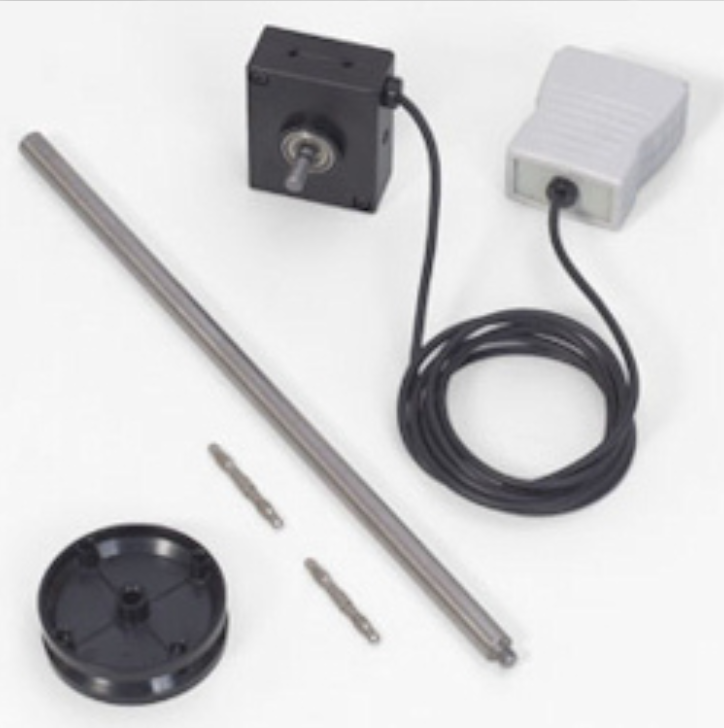
\includegraphics[width=0.5\linewidth]{Figures/IM2.png}
  \caption{Sensor CASSY de movimiento angular.}
  \label{fig:cassy}
\end{figure}


\labday{Miércoles 30, Abril 2025}

\experiment{Construcción del Montaje}

Para la construcción de los péndulos físicos, se utilizaron barras
metálicas obtenidas en el taller de máquinas y herramientas de la
sede Macarena, las cuales cumplían con el requisito previamente
planteado de emplear un material con alta densidad.
Del mismo modo, se avanzó en la preparación del sistema de medición
de ángulos mediante el sensor Cassy, revisando su funcionamiento,
calibración y evaluando la forma de integrarlo al sistema.
Para finalizar, se llevó a cabo la medición de la constante
elástica de los resortes inicialmente seleccionados para la
práctica. Estos resortes fueron adquiridos en una fábrica
especializada con el fin de garantizar constantes elásticas
nominales similares y condiciones físicas consistentes.

\subexperiment{Construcción de los péndulos}
En el taller se identificó una varilla metálica de sección
adecuada. Esta varilla presentaba la rigidez necesaria para
nuestro experimento, por lo que se decidió utilizarla.
A partir de ella, se cortaron las barras con las longitudes
especificadas para el sistema (\(l\) para el central y \(l/2\)
para los laterales). Posteriormente, se pulieron los bordes
para evitar imperfecciones o filos peligrosos, y se perforaron
los orificios necesarios para su montaje.
En el caso de las barras de longitud \(l/2 = \qty{28.0(1)}{\centi\metre}\),
los orificios se realizaron a una distancia de \qty{4.6(1)}{\centi\metre}
desde cada extremo.

Adicionalmente, se midieron las masas de las barras y se determinó
la posición de sus respectivos centros de masa,
medidos desde el punto de pivote. Los resultados se resumen en la
\cref{tab:bars-dat}.

\pgfplotstableread[col sep=comma, header=true]{
	i, y_cm_i, m_i
	1, 14.2, 0600.8
	2, 28.0, 1216.3
	3, 14.0, 0601.8
}\mydata

\begin{table}[htbp!]
	\centering
	\pgfplotstabletypeset[
	col sep=comma,
	zerofill,
	columns/i/.style={
		string type,
		column type={c},
		column name={\(i\)},
	},
	columns/y_cm_i/.style={
		column name={\(y_{\text{cm}_i} [\si{\centi\metre}]\)},
		precision=1,
		fixed,
		fixed zerofill,
	},
	columns/m_i/.style={
		column type={c},
		column name={\(m_i [\si{\gram}]\)},
		dec sep align,
		precision=1,
		fixed,
		fixed zerofill,
	},
	every head row/.style={
		before row=\toprule,
		after row=\midrule,
	},
	every last row/.style={
		after row=\bottomrule,
	}
	]\mydata
	\caption{Parámetros físicos de las barras empleadas en el montaje.
		La incertidumbre para la posición del centro de masa (\(y_{\text{cm}_i}\))
		es de \qty{0.1}{\centi\metre} y para la masa (\(m_i\)) es de
	\qty{0.1}{\gram}.}
	\label{tab:bars-dat}
\end{table}

\begin{figure}[htbp!]
	\centering
	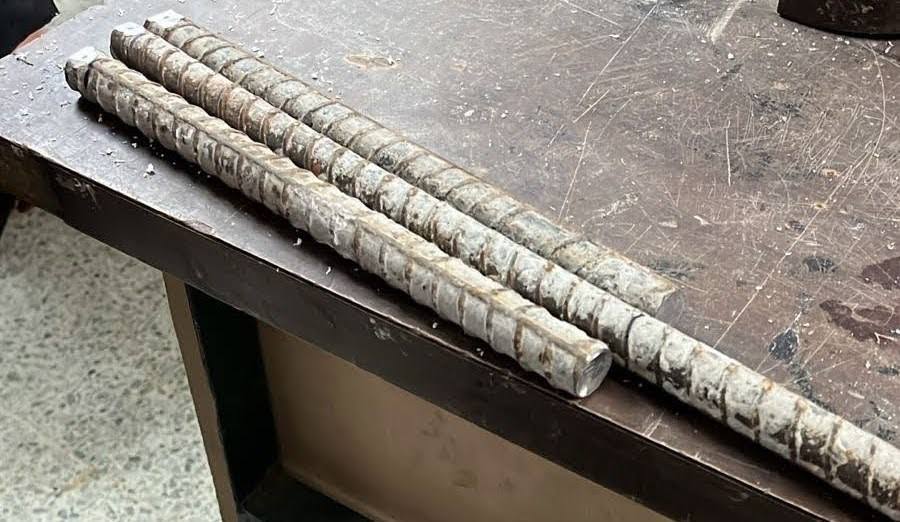
\includegraphics[width=0.7\linewidth]{./Figures/metal-bars.jpeg}
	\caption{Barras metálicas preparadas para el montaje de los péndulos.}
	\label{fig:metal-bars}
\end{figure}

\subexperiment{Preparación del Dispositivo \emph{Cassy}}
Se realizó una revisión inicial del sistema de medición Cassy.
Esta observación permitió definir una estrategia preliminar para
su integración en el sistema, con el fin de registrar los
ángulos de oscilación. Se empleará alambre dulce para fijar las
barras a la rueda giratoria de cada sensor, utilizando los
orificios correspondientes en ambas partes.

\subexperiment{Medición de la constante elástica}
Se llevó a cabo la medición de la constante elástica de los
resortes que se planea utilizar en el experimento. Para esto,
se empleó el montaje experimental convencional de aplicar masas
conocidas a cada resorte, medir su elongación y, mediante una
regresión lineal de desplazamiento en función de la masa soportada,
estimar su constante de elasticidad.

Se utilizaron masas en un rango de \qty{50}{\gram} a \qty{80}{\gram}.
Para dos resortes representativos, se obtuvieron constantes de
elasticidad de \(k_1 = \qty{3.04(4)}{\N\per\m}\) y
\(k_2 = \qty{3.32(6)}{\N\per\m}\). Los valores de desplazamiento
según la masa aplicada se presentan en la \cref{fig:springs-plot}.

\begin{figure}[htbp!]
	\centering
	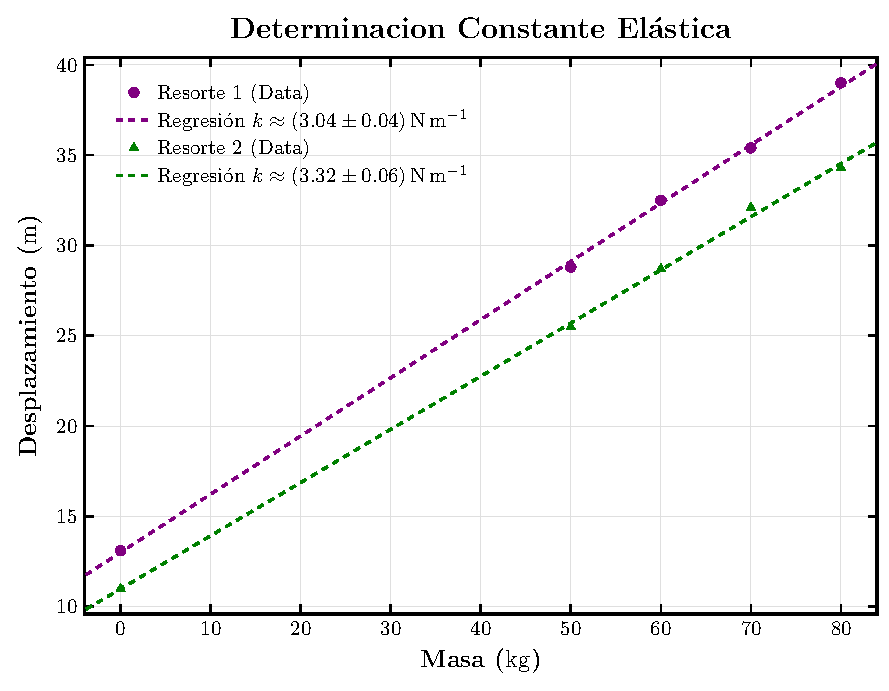
\includegraphics[width=0.6\linewidth]{./Figures/springs-plot.pdf}
	\caption{Determinación de la constante elástica de los resortes.}
	\label{fig:springs-plot}
\end{figure}


\printbibliography

\end{document}
